\chapter{Theoretical Background}\label{chap:background}
% \section{Background and Related Work}
% 3 pages max, i was expecting 
This chapter describes the theory required to understand the proposed solution to the research question. Section \ref{chap:2:compvis} describes briefly the genesis of computer vision, the limitations and the rationale that was followed while developing computer vision techniques. Section \ref{chap:2:machinelearning} introduces the breakthroughs in computer vision thanks to deep learning techniques. Narrowing the scope, section \ref{chap:2:3d} describe the advancements in 3D object recognition and its limitations and section \ref{chap:2:semantic-segmentation} sheds a light on state of the art for object segmentation techniques. Section \ref{chap:2:pose} presents the topic of pose estimation, the current techniques and its limitations. Finally, section \ref{chap:2:summary} summarizes the computer vision timeline and gives an overall idea of the path research has taken up to today for 3D pose estimation. The following questions will be answered in this chapter:
\begin{itemize}
    \item What are the origins of computer vision?
    \item What propelled the development of deep learning techniques in computer vision?
    \item What is the current state of 3D object model estimation techniques?
    \item What is the current state of pose estimation techniques?
\end{itemize}

\section{Traditional Computer Vision Systems}\label{chap:2:compvis}
Computer vision has its origins in the 1960s, when computer models were conceptualized in an attempt to simulate human perception. Back then, computer vision was studied following a "blocks" approach (polyhedra), as introduced by Larry Roberts \cite{huang1996computer}. Later, David Marr proposed a set of required stages for carrying out image understanding. His goal was to reach a 3D understanding of the models in a scene. Figure \ref{fig:marr-stages} illustrates Marr's algorithm to identify the visual world. 


\begin{figure}[!ht]
        \centering
        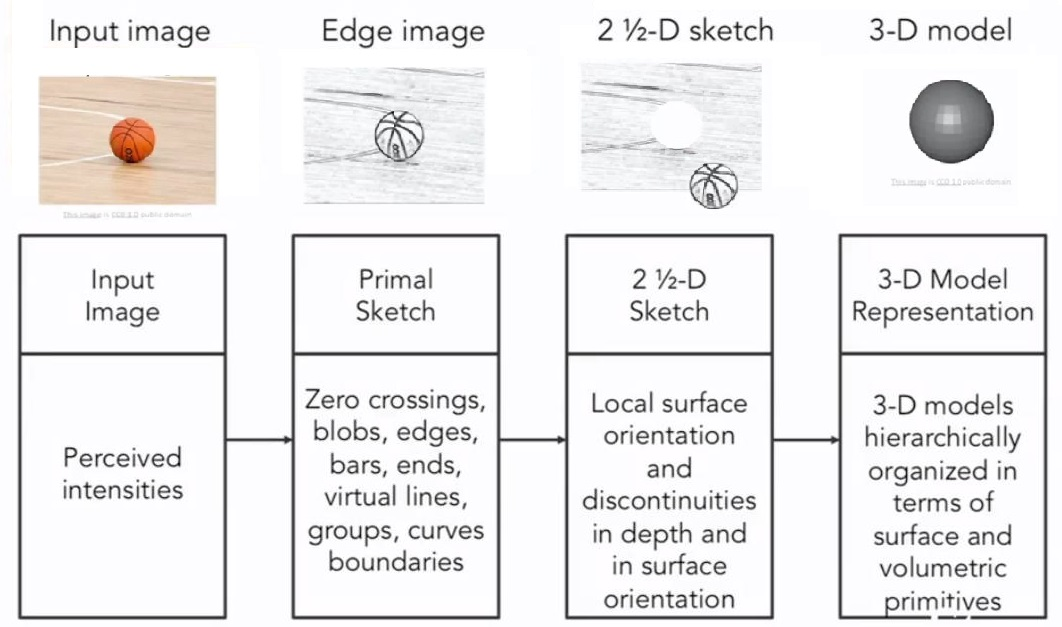
\includegraphics[width=0.72\textwidth]{images/marr-stages}
        \caption{David Marr's stages to identify the visual world.}
        \label{fig:marr-stages}
    \end{figure}
    
Throughout the years, however, most computer vision applications did not require complete 3D object models of the world. Nevertheless, Marr's paradigm shaped the future of computer vision for the years to come. The methods developed until circa 2000 analyzed images in terms of simple geometric features, such as a combination of lines.
% Most of the developed methods manipulated the pixels in images to create features.
The basic initial goal for computer vision was to achieve object segmentation, separating the background from salient objects. Later, the analysis of pixels and more complex features allowed to identify colors, shapes and objects in images. When the same features were seen in multiple images, an image could be classified by approximation. These collection of features for classification was called a "bag of words". Consequently, traditional machine learning approaches such as SVMs, boosting methods and graph models eased the usage of features for classification. Examples of features are:
\begin{itemize}
    \item Scale Invariant Feature Transform (SIFT) \cite{karami2017image}
    \item Speeded Up Robust Features (SURF) \cite{bay2006surf}
    \item Features from Accelerated Segment Test (FAST) \cite{rosten2006machine}
    \item Hough Transforms \cite{goldenshluger2004hough}
    \item Geometric Hashing \cite{tsai1994geometric}

\end{itemize}
Nowadays, traditional computer vision techniques are used in aerospace field, industrial automation, security inspections, intelligent transportation systems, security and transportation systems \citeauthor{bhargava2018fruits} are mostly used to perform simple tasks where machine learning is excessive or in situations where there are memory constraints (microcontrollers). However, machine learning methods for computer vision not only outperform classical computer vision in some tasks, but have also shown progress in classical computer-vision-dominated fields, such as embedded systems, as discussed by \textcite{zhang2019skynet} in \citetitle{zhang2019skynet}. 

%     \begin{itemize}
%         \item one paragraph of ML advancements 1960 - 2010
%         \item one paragraph how these methods are good at image processing but they showed lack of reliability without actually understanding what is in the scene
%     \end{itemize}
\section{Deep Learning for Vision}\label{chap:2:machinelearning}
In 1943, following the ambition of trying to simulate the way the human brain is made up of a collection of simple units, McCulloch and Pitts \cite{mcculloch1943logical} developed a model of a neuron. They called this neuron MCP, which contributed to development of the neural networks we know today. Fast forward to 2010, both public data and GPU hardware availability allowed for the rise of machine learning methods for computer vision. More specifically, the subfield of machine learning, deep learning, leveraged the computing power and data availability for training neural networks with many layers. These deep neural networks could outperform state of the art methods and reach super-human performances. Additionally, an open source project called ImageNet \cite{deng2009imagenet} was born to become one of the largest high-quality public databases for image classification, with the paper \citetitle{krizhevsky2017imagenet} \cite{krizhevsky2017imagenet} being cited over 77000 times as of today. Other breakthroughs, such as the alleviation of the vanishing gradients problem, new regularization techniques and the surge of frameworks for deep learning development, contributed to bringing deep learning to the state we know of today.

\begin{figure}[!ht]
        \centering
        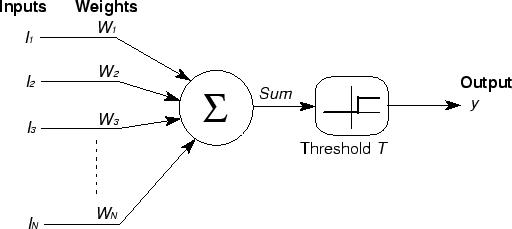
\includegraphics[width=0.5\textwidth]{images/mcculloch-pitts-model.png}
        \caption{McCulloch-Pitts model of a neuron.}
        \label{fig:cow_fmc}
    \end{figure}
    
Over the past 10 years, deep learning has made never-seen-before breakthroughs in a variety of fields such as object detection, semantic segmentation, motion tracking, human pose estimation, and action recognition. Even though some fields have reached a level of maturity, such as 2D object detection, as of today, 3D object recognition remains a challenge.

  


% With the rise of CNNs, the foundation has been set for well-performing image classification approaches such as ResNet [6] or VGG [7]. In recent years, this development has gone even further towards systems which are capable of localizing or even masking out objects in images. Popular approaches with these capabilities are for example Mask R-CNN [9] or YOLO [8]. While using different approaches, both systems have the capability of localizing and semantically classifying objects in images. Mask R-CNN is even able to mask the pixel-areas that are belonging to the object by using polygonal shapes. In the background both approaches still rely on ResNet for feature extraction.

% While systems like these are highly impressive and sufficient for many cases, they are still far away from human visual perception and actual scene understanding [10]. Especially the shortcomings presented in section 1.2 apply to this kind of systems. The resulting polygon-masks or bounding boxes are not projected into 3D space but merely mapped onto the 2D coordinates of the image. If employed on sequential data, both systems would also need to reevaluate the whole frame on each timestep as they are not able to remember or track objects. This is problematic when understanding a scene, as it is often not likely for the whole scene to be visible at once, but only partially. Therefore we believe, it is crucial for a system not to forget but to accumulate information over timesteps.

\section{Semantic Segmentation}\label{chap:2:semantic-segmentation}
Nowadays, computer vision techniques reach human-like performance for localizing and classifying objects in a 2D image. An extension of the recognition problem involves assigning labels to the specific pixels in a given image that belong to the detected objects, instead of only using the bounding boxes obtained during localization. This is called object segmentation, and this section will introduce one the current state of the art methods: MaskRCNN.
% (object segmentation). This section will add to the topic of semantic segmentation. 
% both 2D and 3D object detection attempt to
% Research on object segmentation has built upon the work done in previous image classification models to reach the current state of the art of 2D object segmentation: Mask R-CNN. The image saliency approach each (previous) model takes is described below:
Over the years, object segmentation techniques have tried to improve previous methods, attempting to solve bottle necks and improve both accuracy and speed. The following methods have built upon the previous to reach state of the art performance:
\begin{itemize}
    \item \textbf{R-CNN:} a “selective search” algorithm proposes bounding boxes and features are obtained using a deep convolutional neural network (for example, AlexNet). Object classifications are then made with linear SVMs.
    \item \textbf{Fast R-CNN:} unifies the feature detector, and the bounding box predictor approach into a single model, but the region of interests are still part of the input. The shared computation showed speed improvements.
    \item \textbf{Faster R-CNN:} unifies the region proposal algorithm into the CNN model. This model merges a RPN (region proposal network) with Fast R-CNN.
    \item \textbf{Mask R-CNN:} extends the previous model to add pixel-level image segmentation. A small fully connected network was added that per region of interest outputs a segmentation mask.
\end{itemize}

Understanding these basic overview of these approaches will prove useful for the pipeline this work proposes in the future chapters.
\section{Going into the 3D World}\label{chap:2:3d}
% \lipsum[1-3]
% the same way that iphones rose, smart robots will rise.
% As algorithms and technologies continue to improve over the years, we have witnessed the rise of smartphones, smart homes and now smart offices. 

In their 2020 Hype Cycle for Artificial Intelligence, Gartner projects smart robots to be at their peak of expectations in about 2 to 5 years. This projection goes hand-in-hand with another projection in the same hype cycle. Gartner projects that computer vision will be in the slope of enlightenment around the same period. This is where the experts predict computer vision will enable applications to exploit another input stream: vision. The same way that computers and embedded systems are able to interpret audio and text input from sensors, keyboards, microphones, etc., systems will have access to vision to perform a variety of tasks. 
% n will enable systems to leverage vision for a variety of tasks. 
As \citetext{singh2018fotonnet} describes, "the ability for robots and computers to see and understand the environment is becoming a burgeoning field, needed in autonomous vehicles, augmented reality, drones, facial recognition, and robotic helpers". Since the rise of the CNN \cite{krizhevsky2017imagenet} deep learning based methods for image classification have reached state of the art performance for 2D detection.
% Object localization and segmentation are extensions to the image classification problem, which .
% which current 2D methods can now tackle. 

% In this work the focus is one of the current challenges for computer vision: 3D object recognition. As of today
Nevertheless, 3D scene interpretation methods continue to struggle because of 1) the lack of publicly available RGB-D data sets \cite{han2019image} and 2) the lack of accessibility for developers to hardware \cite{singh2018fotonnet}. These two delaying factors are fortunately slowly changing. First, RGB-D data sets continue to be released to support the development of new algorithms, such as the Mediapipe data set that Google released in November of 2020 \cite{objectron2021dataset}. Second, more and more low-cost 3D image sensors are being made available. The newest smartphones, for example, have been equipped with time-of-flight cameras, not only for photography but also extend their capabilities for AR applications and gaming \cite{tian2019occlusion}. Even though it is still not possible for any RGB-D data set to be as big as the ImageNet data set (∼5 million images), techniques continue to be developed to exploit geometric features and to utilize tools and concepts from 2D methods for 3D visual interpretation.
% available 2D information, new geometric features, etc. 
% Even though 3D labeled data sets are scarce \cite{singh}, this is slowly changing \cite{google}\cite{3ddataset}. Likewise, 3D-depth sensors are not widely available as of today \ref{singh}, but this is slowly changing \ref{cheap-3d-sensors-phone}. 
% to 3D-image sensors in phone 
% due to the growing availability of public large data sets. low-cost 3D image sensors,  in the development phase, due in great part to a lack of publicly available large data sets. 
\textcite{han2019image} provide a thorough review of recent research for 3D object reconstruction. A brief overview of the methods that have been successful at 3D object recognition and reconstruction is presented below:
\begin{itemize}

    \item The majority of works pre-2018 use voxelized representations \cite{yan2016perspective} \cite{choy20163d} \cite{wu2016learning}, which allow the representation of arbitrary topology considering both the surface and the internal structure of object. Representation types of data are: volumetric (based on 3D voxel grids), surface-based (meshes, point clouds) and intermediate (3D reconstruction is done based off 2D information from RGB images).
    \item Since convolutions and overall processing of 3D images has a high memory requirement, volumetric techniques leverage octrees \cite{meagher1980octree}, which are sparse partitioning techniques for 3D grid structures (O-CNN \cite{wang2017cnn}, OGN \cite{tatarchenko2017octree}, OctNet \cite{riegler2017octnet}) to achieve high resolutions while maintaining memory efficiency. As described by \textcite{tatarchenko2017octree}, Octree Generating Networks reduce memory requirements for reconstruction from 4.5 GB to 0.29 GB. These techniques, however, are complex to implement which impacts their reproducibility and further research.
    \item Other approaches learn continuous Signed Distance Functions \cite{park2019deepsdf, chen2019learning} or continuous occupancy grids \cite{mescheder2019occupancy}. These methods have a lower memory requirement and can reconstruct the 3D object at the desired resolution. 
    \item Methods that look at multiple frames for reconstructing representations outperform single-view methods for they collect more information about the silhouette of the objects. 
    \item Techniques that try to reconstruct primarily the surface of a seen object (surface-based techniques) outperform volumetric methods by a small margin. These are: Mesh-based approaches \cite{pontes2018image2mesh} and Point-based approaches \cite{kurenkov2018deformnet, fan2017point}.
    \item Methods that utilize 2D supervision to reconstruct 3D objects improved their performance since 2017, and are outperformed by 3D supervision-based approaches by a small margin. \cite{yan2016perspective, arsalan2017synthesizing}.
\end{itemize} 

    
    
Similarly, \citeauthor{han2019image} provide a set of research directions based on the challenges and limitations that 3D object recognition currently faces. These areas of improvement can be summarized as follows:
\begin{itemize}
    \item Bigger training data sets since deep learning methods depend heavily on them. 
    \item Generalization to unseen objects, and not just specific-domain models.
    \item Methods that allow for 3D reconstruction in higher resolutions, such as reconstruction of hairs, fur and plants.
    \item Combined approaches for both recognition and reconstruction in a single method.
    \item Domain specialized methods that can perform well also on unseen objects, but of a specific domain, say wild animals, which are not easy to label.
    \item Reconstruction of 3D video streams where frames are missing and information is passed from future frames to previous ones.
    \item Full 3D scene understanding, which requires detection, recognition, reconstruction, spatial awareness and robustness to unseen objects.
\end{itemize}
\begin{figure}[!ht]
        \centering
        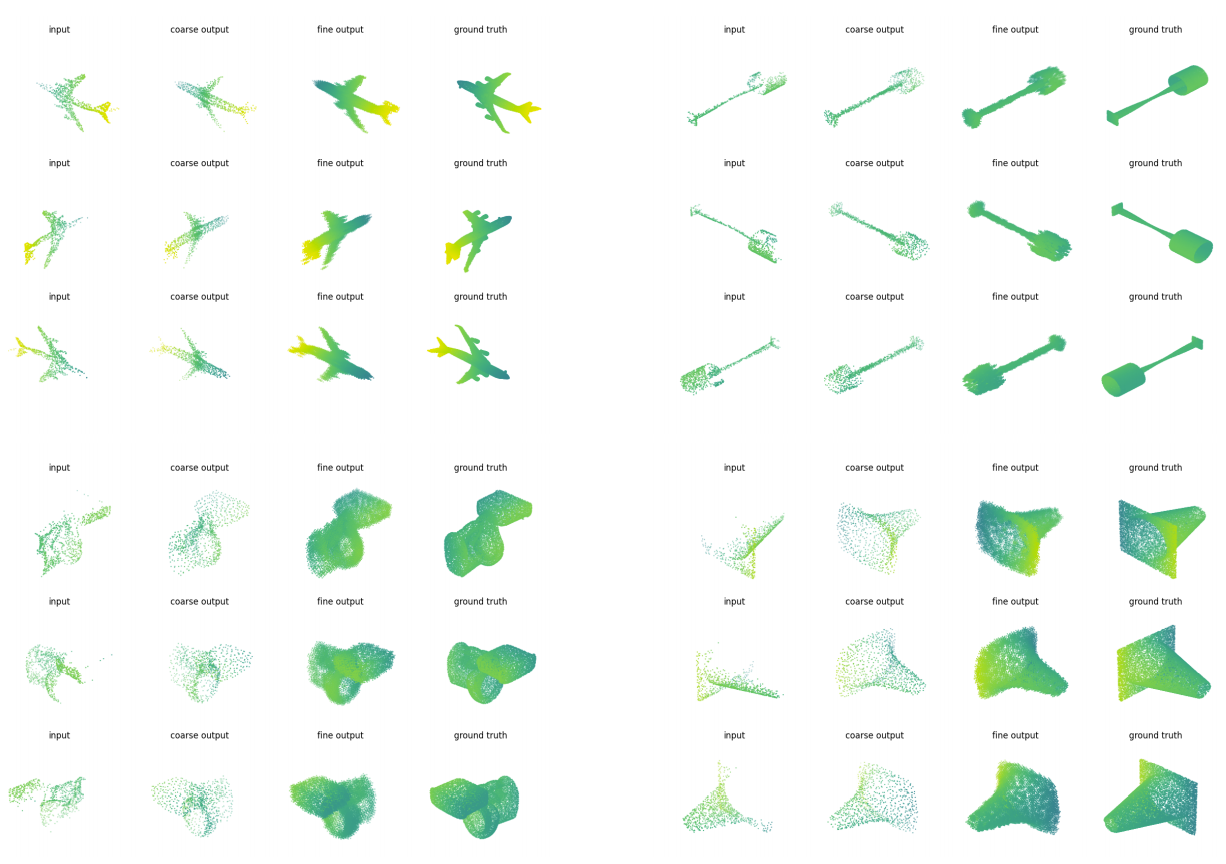
\includegraphics[width=0.8\textwidth]{images/occo-results}
        \caption{Results of using OcCo (2020) pre-training for completion of point clouds.}
        \label{fig:occo-results}
    \end{figure}
    
Along these lines, research from 2020, such as PointContrast \cite{xie2020pointcontrast} and OcCo \cite{wang2020pre} propose pre-training on ShapeNet \cite{chang2015shapenet} to leverage the information contained in point clouds for scene understanding and for reconstructing occluded point clouds respectively. Figure \ref{fig:occo-results} illustrates the performance of OcCo pre-training  for completion of occluded point clouds.


\section{Pose Estimation}\label{chap:2:pose}
Pose estimation is an extension of the 3D object recognition problem. It involves predicting a 3D translation and a 3D rotation. These types of methods have been trained using both synthetic \cite{gupta2015aligning} and real data \cite{li2019gs3d}, labeled with the 6D poses of the objects. Additionally, these methods can be 2D supervision-based or 3D supervision-based. 2D supervision-based methods utilize the information in the RGB image to predict a 3D bounding box, whereas 3D supervision-based methods directly detect 3D bounding boxes from stereo images, RGB-D cameras or LIDAR sensors \cite{sahin2020review}. 
\begin{figure}[!ht]
        \centering
        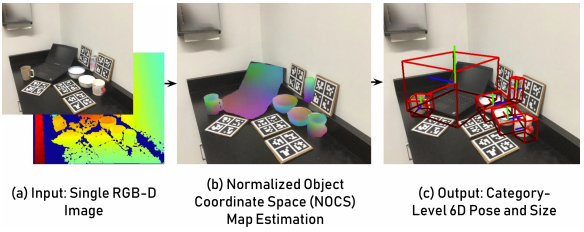
\includegraphics[width=0.7\textwidth]{images/wang-pose}
        \caption{Wang et al. proposed method for category-level 6D pose and
size estimation of multiple unseen objects in an RGB-D image.}
        \label{fig:wang-pose}
    \end{figure}
    
\textcite{sahin2020review} propose a discriminative categorization criteria to organize pose estimation techniques, as follows:
\begin{itemize}
    \item \textbf{Classification-based} approaches leverage 2D information to retrieve a 3D bounding box. Then, a refinement stage is added, such as random forests, to obtain the 6D pose of the object. Examples include: GS3D \cite{li2019gs3d}, Vote3Deep \cite{engelcke2017vote3deep} and the method by \textcite{michel2017global}.
    \item \textbf{Regression-based} approaches are similar to classification based approaches but they run another neural network directly over the predicted 3D bounding box to regress the 6D pose. Examples include: PointFusion \cite{xu2018pointfusion}, FusionNet \cite{hegde2016fusionnet}, VoxelNet \cite{zhou2018voxelnet}, AVOD net [108].
    \item \textbf{Classification and Regression-based} approaches run both tasks mentioned above under the same architecture. Examples include MonoPSR \cite{Ku_2019}, FrustumPNet \cite{qi2018frustum}, PointRCNN \cite{shi2019pointrcnn}, SSD-6D \cite{kehl2017ssd} and DeepContext \cite{zhang2017deepcontext}.
    \item \textbf{Template matching} approaches look at an image using sliding windows and compare obtained features with a database of pre-defined feature templates, and the pose parameter is given to the window with the closest similarity to the template matched. Examples include: the LINEMOD adaptation from \textcite{hinterstoisser2012model}, SVMs embedded in Adaboost \cite{rios2013discriminatively}, RAPID-LR \cite{Munoz_2016} and the method proposed by \textcite{Ku_2018}.
    \item \textbf{Point-pair feature matching} approaches were proposed by \textcite{drost2010model}. The idea is to store point-pair features in a hash table in a separate "offline" stage. During prediction, potential matches then are obtained by comparing to a global model representation. Finally, these matches vote on the pose parameters. These methods underperform given objects with similar features, occlusion and sensor noise \cite{Mohamad_2014}. 
    \end{itemize}


    
Unfortunately, the limitations and challenges mentioned in section \ref{chap:2:3d} overlap with the ones from pose estimation. Along these lines, work by \textcite{Wang_2019} attempts to push pose estimation techniques to being able to generalize to unknown objects, removing the dependency to knowing an object's 3D model previously. Figure \ref{fig:wang-pose} illustrates a glimpse to the method proposed by Wang et al.


% \lipsum[1-3]

    % \begin{itemize}
    %     \item one paragraph of rise of CNNs 2010 - present
    %     \item one paragraph how these methods are not enough for 3d space yet, and importance of not forgetting over timesteps
    % \end{itemize}



    % \begin{itemize}
    %     \item one paragraph about cow robot milking industry
    %     \item ??
    %     \item one paragraph about cow teat morphology 
    % \end{itemize}
% \section{Summary}\label{chap:2:summary}
% % half a page
% \lipsum[1-2]

    % \begin{itemize}
    %     \item one paragraph: describe popular approaches briefly, and main ways literature does it
    %     \item 1P: highlight most interesting literature approach
    %     \item 1P: lastly, we discuss how X is done, and whether it is feasible to extend our approach (prob a small filler?)
    % \end{itemize}
